\subsection{Recap: Quality Assurance}
\begin{frame}{Recap: Software Quality} % caution: slide copied from testing lecture
	\rightorleft{
		\mydefinition{Quality \mysource{\ludewiglichter}}{Quality is the entirety of properties and characteristics of a product or process that indicate adequacy with respect to given requirements.}
		\mydefinition{Quality Assurance \mysource{\ludewiglichter}}{Quality assurance \deutsch{Qualitätssicherung} are all activities with the goal to improve the quality.}
	}{
		\vspace{-12mm}
		\href{https://commons.wikimedia.org/wiki/File:Andy_Hunt_programmer.jpg}{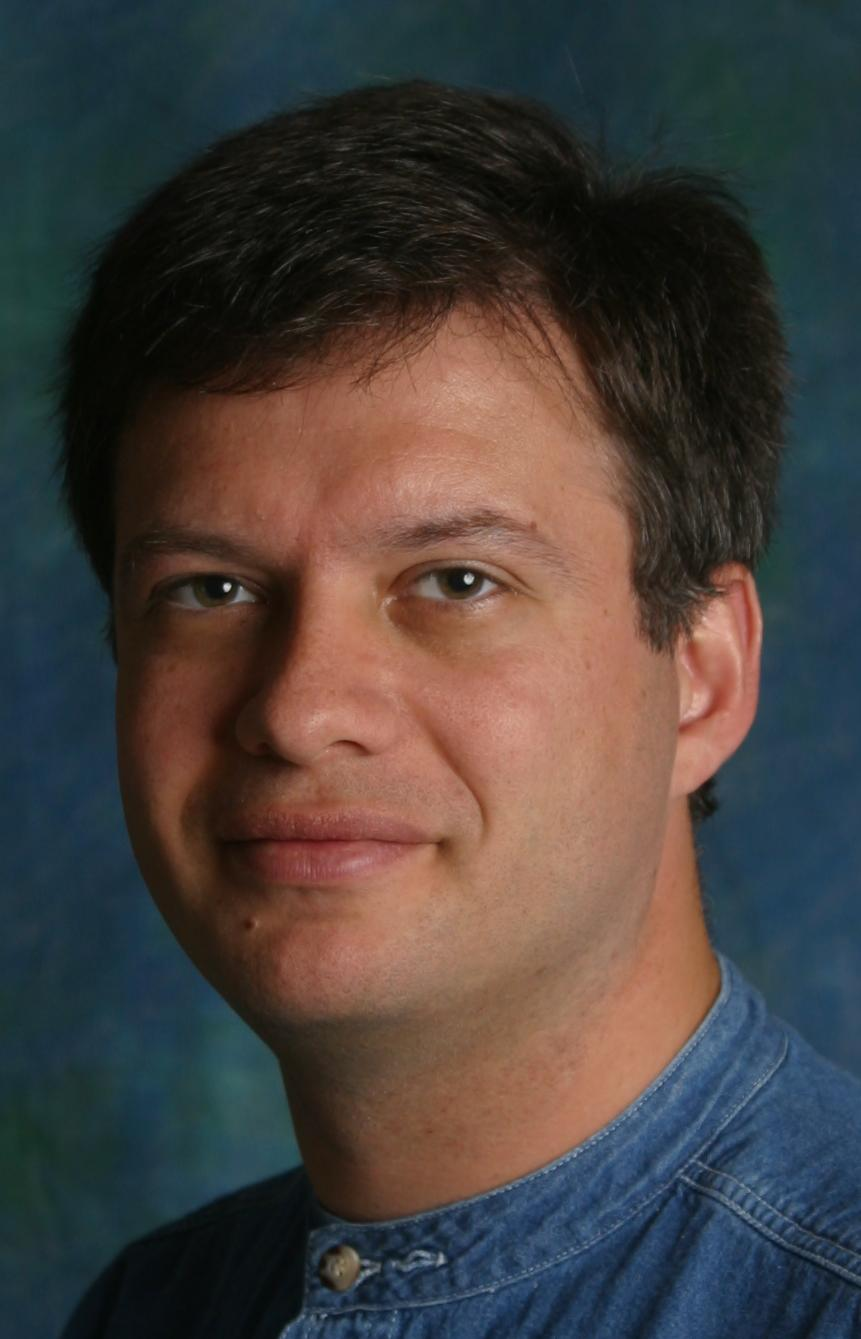
\includegraphics[width=\linewidth,trim=0 240 0 300,clip]{andy-hunt}}
		\vspace{-7mm}
		
		\mynote{Andy Hunt \mysource{\thepragmaticprogrammer}}{\mycite{No one in the brief history of computing has ever written a piece of perfect software. It's unlikely that you'll be the first.}}
		% co-authored The Pragmatic Programmer, known for the Agile Manifesto
	}
\end{frame}

\begin{frame}{Recap: Quality Assurance \mytitlesource{\ludewiglichter}} % caution: slide copied from testing lecture
	\hfill%
	\only<1|handout:0>{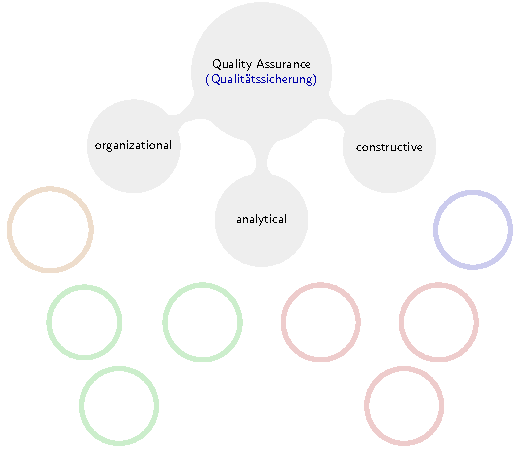
\includegraphics[height=\textheightwithtitle,page=1]{quality-assurance}}%
	\only<2|handout:0>{\includegraphics[height=\textheightwithtitle,page=2]{quality-assurance}}%
	\only<3|handout:0>{\includegraphics[height=\textheightwithtitle,page=3]{quality-assurance}}%
	\only<4|handout:0>{\includegraphics[height=\textheightwithtitle,page=4]{quality-assurance}}%
	\only<5|handout:1>{\includegraphics[height=\textheightwithtitle,page=5]{quality-assurance}}%
	\only<6|handout:0>{\includegraphics[height=\textheightwithtitle,page=6]{quality-assurance}}%
	% TODO check why this mindmap has a white background. could be large without a white background when using \textheightwithouttitle
\end{frame}

%mit nem emotionalen Bild motivieren => gute Softwarequalität ist wichtig

% mit quadranten starten
%bezug auf FM-analyse
%wir gucken uns jetzt Source Code an (evtl. linke zwei (VL 4, Problem Space) + rechte zwei Quadranten (VL 10+, Solution Space))
% wechselwirkung zw. sol und problem space (mapping+FM)

% properties one might want to analyze, similar to questions about feature models in modeling.tex
% include questions for all four quadrants

%zB Lego-Beispiel verwenden?

%strategien high-level angucken
%product-based
%number crunching, wie groß sind SPLs, product-based skaliert nicht

%ich könnte weniger produkte angucken (sampling)
%grundstein für test-vorlesung

%oder nur features angucken: feature-based
%wichtige message: es reicht nicht, features einzeln zu analysieren
%rückgriff auf interaktionen (dass feature-based nicht reicht)

%feature-product

%family (motivieren)

\subsection{Asking Questions About Product Lines}

\subsection{Classification of Product-Line Analyses (SPLE?)}

\subsection{Classification of Product-Line Analyses (CSUR? im 3. Block?)}

\subsection{Complexity of Product Lines}
\begin{frame}{\insertsubsection}
	\leftorright{
		\mydefinition{Product-Line Complexity Classes}{
			In a timeframe of 24h \ldots
			\begin{enumerate}
				\item[C0] Products cannot be generated automatically
				\item[C1] All products can be tested
				\item[C2] Not C1, but all products can be generated
				\item[C3] Not C2, but all configurations can be generated (aka. ALLSAT)
				\item[C4] Not C3, but the number of valid configurations can be computed (aka. \#SAT)
				\item[C5] Not C4, but whether there is a valid configuration can be computed (aka. SAT)
				\item[C6] It cannot be computed whether there is a valid configuration
			\end{enumerate}
		}
	}{
		\myexample{Examples}{
			\begin{enumerate}
				\item[C0] all product lines with custom development in application engineering\\(e.g., components and services with glue code, white-box frameworks)
				\item[C1] $< 2,000$ products for 1 min per product
				\item[C2] $< 90,000$ products for 1 s per product
				\item[C3] $< 10^{13}$ configurations for 1 ns per configuration
				\item[C4] older versions of Linux/Automotive05
				\item[C5] newer versions of Linux/Automotive05\\(see \evaluatingsharpsatsolvers)
				\item[C6] No example known
			\end{enumerate}
		}
	}
\end{frame}
